\section{Space complexity}
\label{sec:space}

We prove that the BHF achieves the information-theoretic lower bound on space
complexity for both Bernoulli sets and Bernoulli maps, under both predicate
forms.

\subsection{General proof (maps)}

The BHF representation is the tuple $(h_k, b)$ or $(N, t, b)$.
The dominant term is the length of the salt $b$, which the algorithm discovers
by exhaustive search in order of increasing length.

\begin{theorem}[Success probability per trial]
\label{thm:success_prob}
The probability that a candidate salt $b$ yields a valid BHF for a map with
$m$ keys, false positive rate $\fprate$, and mean value encoding length $\mu$
is:
\begin{enumerate}[(i)]
    \item Equality predicate: $p_{\mathrm{eq}} = \fprate^{m-1} / 2^{m\mu}$.
    \item Threshold predicate: $p_{\mathrm{th}} = \fprate^{m} / 2^{m\mu}$.
\end{enumerate}
\end{theorem}
\begin{proof}
See \cref{thm:success_eq,thm:success_thresh}.
\end{proof}

\begin{theorem}[Space complexity of the BHF]
\label{thm:space}
The expected bit length of the BHF asymptotically achieves
\begin{equation}
    -\log_2 \fprate + \mu \;\; \si{bits \per element}
\end{equation}
as $m \to \infty$, for both predicate forms.
\end{theorem}
\begin{proof}
The algorithm searches through candidate salts in order of increasing bit
length.
By \cref{def:mapping}, the \nth candidate maps uniquely to a bit string.
The search terminates at the first success, which follows a geometric
distribution with parameter $p$ (where $p = p_{\mathrm{eq}}$ or
$p = p_{\mathrm{th}}$).

Let $\RV{Q} \sim \geodist(p)$ be the trial at which the first success occurs.
The salt bit length is $\RV{N} \approx \log_2 \RV{Q}$ (a slight overestimate
from dropping the floor).

We approximate $\Expect{\RV{N}}$ via a second-order Taylor expansion of
$\log_2$ around $\Expect{\RV{Q}}$:
\begin{equation}
    \Expect{\RV{N}} \approx \log_2 \Expect{\RV{Q}}
        - \frac{\log_2 e}{\Expect{\RV{Q}}} \Var{\RV{Q}}\,.
\end{equation}
For $\RV{Q} \sim \geodist(p)$, $\Expect{\RV{Q}} = 1/p$ and
$\Var{\RV{Q}} = (1-p)/p^2$.
Substituting:
\begin{equation}
    \Expect{\RV{N}} \approx -\log_2 p + (1 - 1/p) \log_2 e\,.
\end{equation}

\paragraph{Equality predicate.}
With $p = \fprate^{m-1}/2^{m\mu}$:
\begin{align}
    \Expect{\RV{N}}
        &\approx -(m-1)\log_2 \fprate + m\mu
            + (1 - \fprate^{-(m-1)} 2^{m\mu}) \log_2 e\,.
\end{align}
Dividing by $m$ and taking $m \to \infty$:
\begin{equation}
    \frac{\Expect{\RV{N}}}{m} \to -\log_2 \fprate + \mu\,.
\end{equation}

\paragraph{Threshold predicate.}
With $p = \fprate^{m}/2^{m\mu}$:
\begin{align}
    \Expect{\RV{N}}
        &\approx -m\log_2 \fprate + m\mu
            + (1 - \fprate^{-m} 2^{m\mu}) \log_2 e\,.
\end{align}
Dividing by $m$ and taking $m \to \infty$:
\begin{equation}
    \frac{\Expect{\RV{N}}}{m} \to -\log_2 \fprate + \mu\,.
\end{equation}
In both cases, the expected bits per element converges to the information-theoretic lower bound $-\log_2 \fprate + \mu$.
\end{proof}

\subsection{Set as corollary}

\begin{corollary}[Space complexity for sets]
\label{cor:set_space}
For a Bernoulli set ($\mu = 0$), the BHF achieves $-\log_2 \fprate$ bits per
element asymptotically.
\end{corollary}
\begin{proof}
Set $\mu = 0$ in \cref{thm:space}.
\end{proof}

\subsection{Finite-sample correction}

For finite $m$, the exact bits per element are:
\begin{equation}
    \frac{\Expect{\RV{N}}}{m} =
    \begin{cases}
        -\dfrac{m-1}{m}\log_2 \fprate + \mu + \mathcal{O}(1/m)
            & \text{(equality)}\,,\\[8pt]
        -\log_2 \fprate + \mu + \mathcal{O}(1/m)
            & \text{(threshold)}\,.
    \end{cases}
\end{equation}
The equality predicate is slightly more space-efficient for small $m$
(by $\log_2 \fprate / m$ bits per element) due to the adaptive $h_0$.

\subsection{Effect of false negatives}

When $\fnrate > 0$, only $p = (1-\fnrate)m$ elements need to be accepted.
The success probability becomes (for the equality predicate):
\begin{equation}
    p = \frac{\fprate^{p-1}}{2^{p\mu}}\,,
\end{equation}
and the space complexity per element of the \emph{original} set becomes:
\begin{equation}
    \frac{p}{m}\left(-\log_2 \fprate + \mu\right)
    = (1 - \fnrate)\left(-\log_2 \fprate + \mu\right)\,,
\end{equation}
matching the lower bound in \cref{post:map_lb}.

\subsection{Space complexity of the adaptive threshold}
\label{sec:adaptive_space}

The adaptive threshold stores the pair $(N, t)$ with no salt.
This yields dramatically lower per-element cost, but the FPR is a random
variable rather than a fixed parameter.

\begin{theorem}[Space complexity---adaptive threshold]
\label{thm:adaptive_space}
For a Bernoulli set ($\mu = 0$) with $m$ keys and modulus $N$, the adaptive
threshold BHF stores $(N, t)$ using
\begin{equation}
\label{eq:adaptive_bits}
    \lceil \log_2 N \rceil + \lceil \log_2 N \rceil
    \;=\; 2\lceil \log_2 N \rceil \;\;\si{bits}
\end{equation}
total (or $\lceil \log_2 N \rceil + \lceil \log_2(t+1) \rceil$ if $t$ is
encoded in fewer bits).
The per-element cost is
\begin{equation}
\label{eq:adaptive_per_element}
    \frac{2\lceil \log_2 N \rceil}{m} \;=\; \mathcal{O}\!\left(\frac{\log N}{m}\right) \;\to\; 0
    \quad\text{as } m \to \infty\,.
\end{equation}
\end{theorem}
\begin{proof}
The modulus $N$ requires $\lceil \log_2 N \rceil$ bits to encode, and the
threshold $t \in \{0,\ldots,N-1\}$ requires at most $\lceil \log_2 N \rceil$
bits.
There is no salt to store (for sets, $b = \epsilon$).
The per-element cost is the total divided by $m$, which vanishes as
$m \to \infty$ for any fixed $N$.
\end{proof}

\begin{remark}[Why zero per-element cost does not violate the lower bound]
\label{rem:lb_not_violated}
The information-theoretic lower bound of $-\log_2 \fprate + \mu$ bits per
element assumes a \emph{fixed, predetermined} false positive rate $\fprate$.
The adaptive threshold does not fix $\fprate$---it is a random variable
(\cref{thm:fpr_distribution}).
The lower bound applies to the \emph{worst-case} FPR realization, not to
the expected FPR.
More precisely, the adaptive threshold trades FPR
\emph{predictability} for space savings: instead of guaranteeing
$\fprate = \epsilon^{*}$, it guarantees only
$\Expect{\fprate} = p/(m+1) \approx \epsilon^{*}$, with the actual FPR
drawn from a $\betadist(p, m - p + 1)$ distribution whose variance is
$\mathcal{O}(1/m)$.
The ``missing'' $m(-\log_2\fprate)$ bits of information are encoded in the
randomness of $\fprate$ itself.
\end{remark}

\Cref{fig:space_comparison} compares the per-element space cost across the
three predicates.

\begin{figure}[ht]
\centering
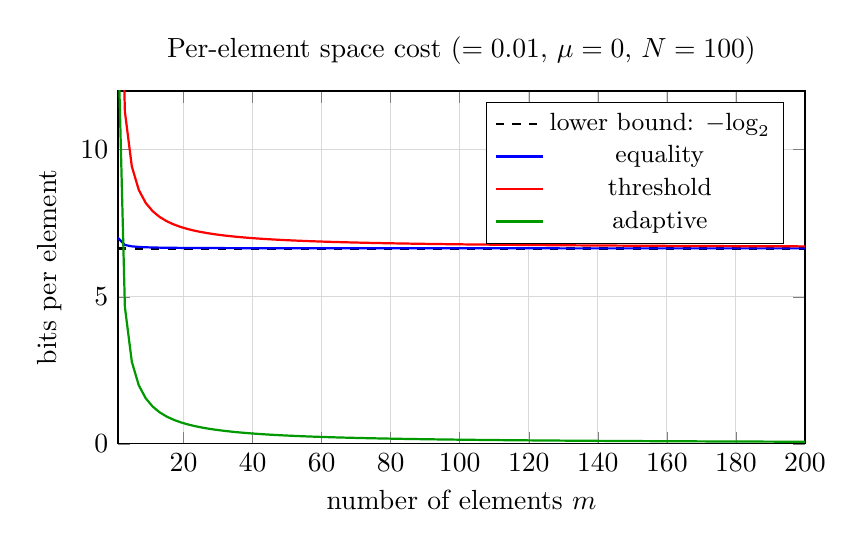
\begin{tikzpicture}
\begin{axis}[
    width=0.85\textwidth,
    height=0.5\textwidth,
    xlabel={number of elements $m$},
    ylabel={bits per element},
    xmin=1, xmax=200,
    ymin=0, ymax=12,
    legend style={at={(0.97,0.97)}, anchor=north east, font=\small},
    grid=major,
    grid style={gray!30},
    every axis plot/.append style={thick},
    title={Per-element space cost ($\fprate = 0.01$, $\mu = 0$, $N = 100$)}
]

% Lower bound: -log2(0.01) = 6.644
\addplot[black, dashed, domain=1:200, samples=100] {6.644};
\addlegendentry{lower bound: $-\!\log_2 \fprate$}

% Equality: -(m-1)/m * log2(eps) + O(1/m) ≈ (m-1)/m * 6.644 + log2(1/eps)/m
% success prob = eps^(m-1), salt bits ≈ (m-1)*log2(1/eps), plus k = log2(1/eps)
% total/m = (m-1)/m * 6.644 + 6.644/m = 6.644
% But for small m, the k bits overhead matters: (k + salt)/m
% k = ceil(log2(1/eps)) = 7 for eps=0.01
% salt ≈ (m-1)*6.644 bits
% total = 7 + (m-1)*6.644, per-element = 7/m + (m-1)/m*6.644
\addplot[blue, domain=1:200, samples=100] {7/x + (x-1)/x * 6.644};
\addlegendentry{equality}

% Threshold: salt ≈ m*6.644, plus ceil(log2 N) + ceil(log2 N) overhead
% total = 14 + m*6.644, per-element = 14/m + 6.644
\addplot[red, domain=1:200, samples=100] {14/x + 6.644};
\addlegendentry{threshold}

% Adaptive: 2*ceil(log2 N) / m = 14/m
\addplot[green!60!black, domain=1:200, samples=100] {14/x};
\addlegendentry{adaptive}

\end{axis}
\end{tikzpicture}
\caption{Per-element space cost for the three BHF predicates with target
    $\fprate = 0.01$ ($N = 100$).
    The equality and threshold predicates converge to the
    information-theoretic lower bound $-\log_2\fprate \approx 6.64$ bits per
    element.
    The adaptive threshold costs $\mathcal{O}(\log N / m) \to 0$ bits per
    element because no salt is stored, but the FPR is a random variable
    rather than a fixed parameter.}
\label{fig:space_comparison}
\end{figure}
